%%%%%%%%%%%%%%%%%%%%%%%%%%%%%%%%%%%%%%%%%%%%%%%%%%%%%%%%%%%%%%%%%%%%%%%%%%%%%%%
%                        MEC3441 eleventh handout 1994.                       %
%%%%%%%%%%%%%%%%%%%%%%%%%%%%%%%%%%%%%%%%%%%%%%%%%%%%%%%%%%%%%%%%%%%%%%%%%%%%%%%
\documentclass[a4paper,11pt]{article} \pagestyle{plain}

\usepackage{amsmath,amssymb,amsxtra,bm,natbib,graphicx,epic,eepic,textcomp}

\graphicspath{{./Figs/}} 

\setlength{\textheight}			{245mm}
\setlength{\textwidth}			{165mm}
\setlength{\topmargin}			{-5mm}
\setlength{\headsep}			{0mm}
\setlength{\oddsidemargin}		{0mm}
\setlength{\parsep}                     {0mm}

\renewcommand{\baselinestretch}		{1.00}

\newcommand{\sss}{\subsubsection}
\newcommand{\qitem}[1]{\refitem {\bf (#1)}}

\input{hmb.mac}

%%%%%%%%%%%%%%%%%%%%%%%%%%%%%%%%%%%%%%%%%%%%%%%%%%%%%%%%%%%%%%%%%%%%%%%%%%%%%%%
\begin{document}
  \biomedsubject{421286}{Bioengineering Systems 2}{2006}

%%%%%%%%%%%%%%%%%%%%%%%%%%%%%%%%%%%%%%%%%%%%%%%%%%%%%%%%%%%%%%%%%%%%%%%%%%%%%%%
\section*{Pipe flow laboratory}

%==============================================================================
\subsection*{Introduction}

This experiment is designed to familiarise you with two central
features of steady flow in pipes: (\textit{i}) the \oned\ energy
equation; (\textit{ii}) the Moody chart (see figure~\ref{fig.moody}),
which is a graphical summary of many experiments on energy losses from
viscous friction in straight pipe flow. Two pieces of equipment will
be employed: (\textit{i}) a pipe flow rig with piezometric tappings
(see figure~\ref{fig.tank}); (\textit{ii}) a simple siphon (see
figure~\ref{fig.siphon}). In both cases, gravitational potential
energy provides the driving force, and the flow rate is determined by
the rate of frictional conversion of kinetic energy, ultimately to
thermal energy. You will compute the (dimensionless) friction losses
and Reynolds number, and compare the values for the losses in the pipe
sections with values on the Moody chart.


%==============================================================================
\subsubsection*{One-dimensional steady-flow energy equation}

When flows are effectively one-dimensional (so that any spatial
variation may be considered to depend only on change in postion along
a line or curve), and where heat transfer and external work sources
(\eg pumps) are absent, the change in energy per unit weight possessed
by a fluid between an upstream location (1) and a downstream location
(2) can be written as:
\begin{equation}
\frac{p_1}{\rho\cg} + \frac{V_1^2}{2\cg} + z_1 = 
\frac{p_2}{\rho\cg} + \frac{V_2^2}{2\cg} + z_2 +
h_\mu
\label{eq.nrg}
\end{equation}
where $p$ is pressure, $\rho$ is fluid density, $\cg$ is the
gravitational acceleration, $V$ is velocity, $z$ is elevation in the
gravity field, and $h_\mu$ represents frictional losses. Note that in
this form, all terms in the equation have units of length. If the flow
has no friction, then the term $h_\mu$ disappears, and the equation is
known as Bernoulli's equation. All real flows (and those in this
laboratory session) have some friction.

Along a length $L$ of pipe with constant diameter $D$, (so that the
flow speed $V$ is constant) the frictional losses are usually
represented as the sum of losses dues to wall friction, and `point'
losses at fitting (entries, exits, bends, valves). And we write
\begin{equation}
h_\mu = \frac{V^2}{2\cg}\left(\frac{fL}{D}+\sum K\right),
\label{eq.loss}
\end{equation}
where $f$ is a dimensionless friction factor and $\sum K$ represents
the sum of dimensionless fitting losses along the length of pipe.

To use this equation, we imagine a steady flow streamline locating one
station and another, \eg between pressure tapping~1 and tapping~2 in
figure~\ref{fig.tank}, or between the free surface in the head tank
(where the flow speed is effectively zero) and tapping~7. Also, we
could draw a `streamline' between one of the pressure tappings, along
the attached piezometer tube to the free surface at its end\,---\,in
this case, the flow speed is zero along the length of tube, and so
using equation~(\ref{eq.nrg}), the change in height is related
directly to the increase in pressure from atmosphere to the pressure
inside the pipe.

Using equations (\ref{eq.nrg}) and~(\ref{eq.loss}), we can compute the
friction loss coefficient $f$ along any single length of pipe, (say
between tapping~1 and~2 or~3 and~4), or the fitting loss coefficient
$K$ for any of the fittings (\eg for the valve between tappings~5
and~6), by measuring the flow rate, hence $V$, and using the
indication of differential pressure inside the pipe from the
differences in heights of at the associated piezometers.

%==============================================================================
\subsection*{Gravity feed straight pipe rig}

In straight pipe rig (see figure~\ref{fig.tank}, water flows from a
constant head tank along a plastic pipe, ID 23.4mm, which has a number
of fittings. The flow rate is regulated with a valve, see
figure~\ref{fig.valve}\,(\textit{a}). The pressure at various points
along the pipe is obtained by means of piezometers: as explained
above, the difference in heights of water at the free surfaces of the
piezometer tubes reflects the difference in pressure within the pipe.

\begin{figure}
\begin{center}
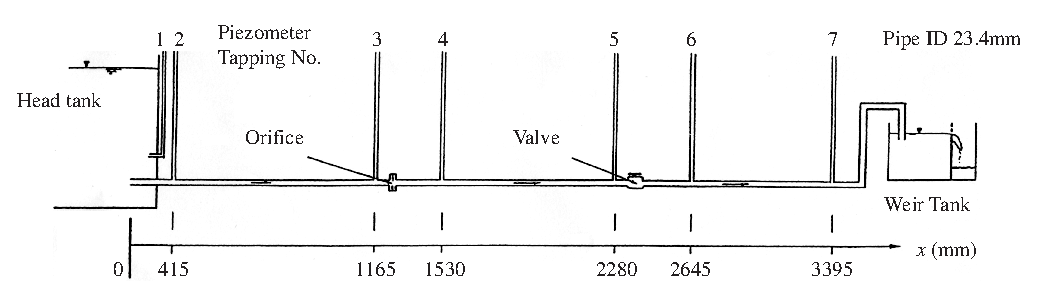
\includegraphics[width=0.9\textwidth]{ExptTankPipeLabel.eps}
\end{center}
\caption{Schematic of pipe flow experiment.}
\label{fig.tank}
\end{figure}

The rate of flow of water through the rig is estimated from the height
of water as it flows over the V-notch weir in the weir tank using an
experimentally determined correlation. See
figure~\ref{fig.valve}\,(\textit{b}). Given the height $H$ \emph{in
metres}, the flow rate of water over the weir $Q$ \emph{in cubic
metres per second} is given by
\begin{equation}
Q=1.485 H^{2.5}.
\label{eq.weir}
\end{equation}
Note that since the equation is otherwise dimensionally inconsistent,
the constant is not dimensionless (what are its units?).

\begin{figure}
\begin{center}
\begin{tabular}{cccc}
(\textit{a}) &
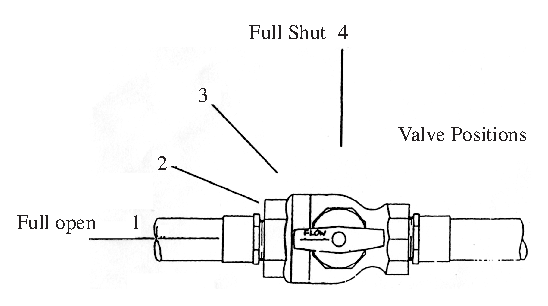
\includegraphics[width=0.45\textwidth]{ExptTankValveLabel.eps} &
\hspace*{2em}
\raisebox{6ex}{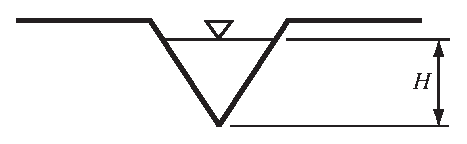
\includegraphics[width=0.35\textwidth]{VNotchWeir.eps}} &
(\textit{b})
\end{tabular}
\end{center}
\caption{Pipe flow experiment: (\textit{a}), valve positions;
  (\textit{b}) height differential $H$ for V-notch weir.}
\label{fig.valve}
\end{figure}

\subsubsection*{Operating procedure}
\begin{enumerate}
\item
With the valve closed (position 4), record the fluid heights in the
piezometer. Using the vernier, record the relative elevation of the
bottom of the V-notch weir.
\item
With the valve opened fully (position 1) again record all the
piezometer heights, and also the relative elevation of the water
upstream of the weir (say 100mm upstream\,---\,why?).
\item
Repeat step 2 for valve openings 2 and 3.
\end{enumerate}

\subsubsection*{Data reduction}
\begin{enumerate}
\item
For each of the three flow rates, use equation~(\ref{eq.weir}) to
compute the volumetric flow rate $Q$ and hence the average flow
velocity in the pipe $V=Q/A=4Q/\pi D^2$. Then also compute the
Reynolds number for each flow rate: $\Rey=\rho VD/\mu=VD/\nu$, where
$\rho$ is the density and $\mu$ the viscosity of water, which are
often combined in the \emph{kinematic viscosity} $\nu$.
\item
From the piezometer readings at each flow rate, compute the friction
factor in each of the three straight lengths of pipe (\ie from
piezometers 2 and 3, then 4 and 5, finally 6 and 7) using
equation~(\ref{eq.loss}).
\item
From the piezometer height differentials 1--2, 3--4, 5-6 at each
flowrate, calculate the loss coefficients $K$ for these fittings: pipe
entry, orifice, and valve. Note that the head drop from 1--2 results
from both a change in velocity (since the velocity is effectively zero
at station 1) and the frictional fitting loss associated with flow
separation in the pipe entry.
\end{enumerate}

%==============================================================================
\subsection*{Siphon rig}

You will use a siphon (see figure~\ref{fig.siphon}) to transfer water
from a higher location (a graduated cylinder) to a lower one (a
bucket) through plastic tubes.

\subsubsection*{Procedure}
There must be enough water in the graduated cylinder and bucket to
keep each end of the tube submerged.  For each size of tube:
\begin{enumerate}
\item
Record the length and internal of the tube.
\item
Initiate flow through the tube as shown by the demonstrator, submerge
the top end of the tube in the graduated cylinder. Now use a stopwatch
to record how long it takes to drain a known volume of fluid. Stop the
flow by exposing the top end of the tube.
\item
Use a ruler to measure the average height differential $H$ between the
fluid level in the graduated cylinder and that in the bucket.
\end{enumerate}

\begin{figure}
\begin{center}
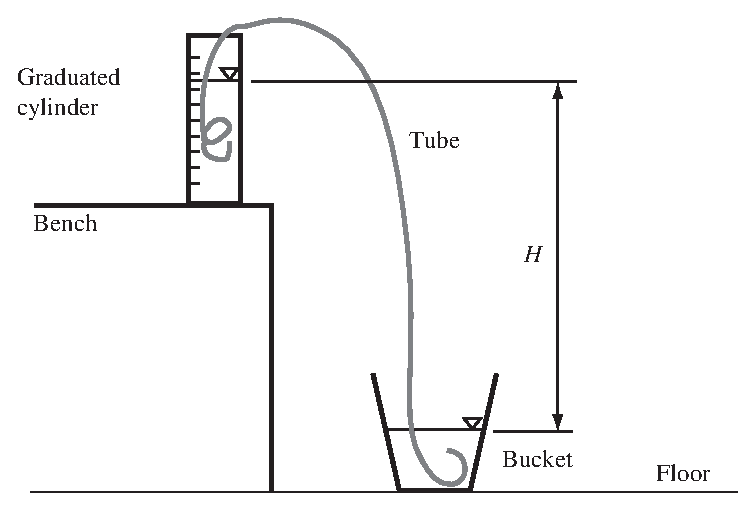
\includegraphics[width=0.5\textwidth]{Siphon.eps}
\end{center}
\caption{Schematic of siphon experiment with free surface height
  differential $H$.}
\label{fig.siphon}
\end{figure}

\subsubsection*{Data reduction}
For each size of tube:
\begin{enumerate}
\item
Compute the flow rate $Q$, average speed $V$ and the Reynolds number,
$\Rey$.
\item
Using assumed loss coefficients $K=0.75$ for the tube entry flow and
$K=1$ for the tube exit flow, use equations~(\ref{eq.nrg})
and~(\ref{eq.loss}) to compute the pipe flow fricton factor $f$.
\end{enumerate}

%==============================================================================
\subsection*{Report}

You must submit a formal written report on your findings for
assessment. The idea is to provide a record that would allow someone
else to (\textit{a}) understand what was done and the main outcomes;
(\textit{b}) if necessary to repeat the experiment on their own;
(\textit{c}) follow and check your calculations.

\begin{enumerate}
\item
Supply your name, the title of the experimental session, the date, and
the names of the others in your group.
\item
For both the straight pipe rig and the siphon, tabulate the readings
recorded in the experimental section (piezometer heights, weir
heights, tube diameter, length, volume transferred, time taken,
etc.). Give SI units for all quantities.
\item
Provide an example calculation for each of the derived quantities
($Q$, $V$, $\Rey$, $K$, $f$, etc.). Give SI units for all dimensional
quantities and calculated results (where appropriate).
\item
For both the straight pipe rig and the siphon, supply a tabulated
summary of the derived quantities.  For the straight pipe rig, supply
the values of the loss coefficients for each of the fittings, averaged
over the three flow rates ($K$ is approximately independent of
Reynolds number). Also for this rig, note that at each valve opening,
there will be three values of $f$, one for each section of pipe 2--3,
4--5, 6--7. Tabulate also the average of these three at each flow rate
($f$ is not independent of $\Rey$).
\item
On the attached Moody chart (figure~\ref{fig.moody}), plot the three
average $f$ values for the straight pipe flow experiment, and the two
values for the siphon experiment.
\item
Provide a brief summary of the experiment and your findings. Compare
the loss coefficients for the various fittings with values supplied in
fluid mechanics textbooks. Comment on the comparison between the
values of friction factor $f$ that you derived and those on the Moody
chart, and give your assessment as to the major contributing factors
in any differences highlighted in this comparison.
\end{enumerate}

\newpage
\begin{figure}
\begin{center}
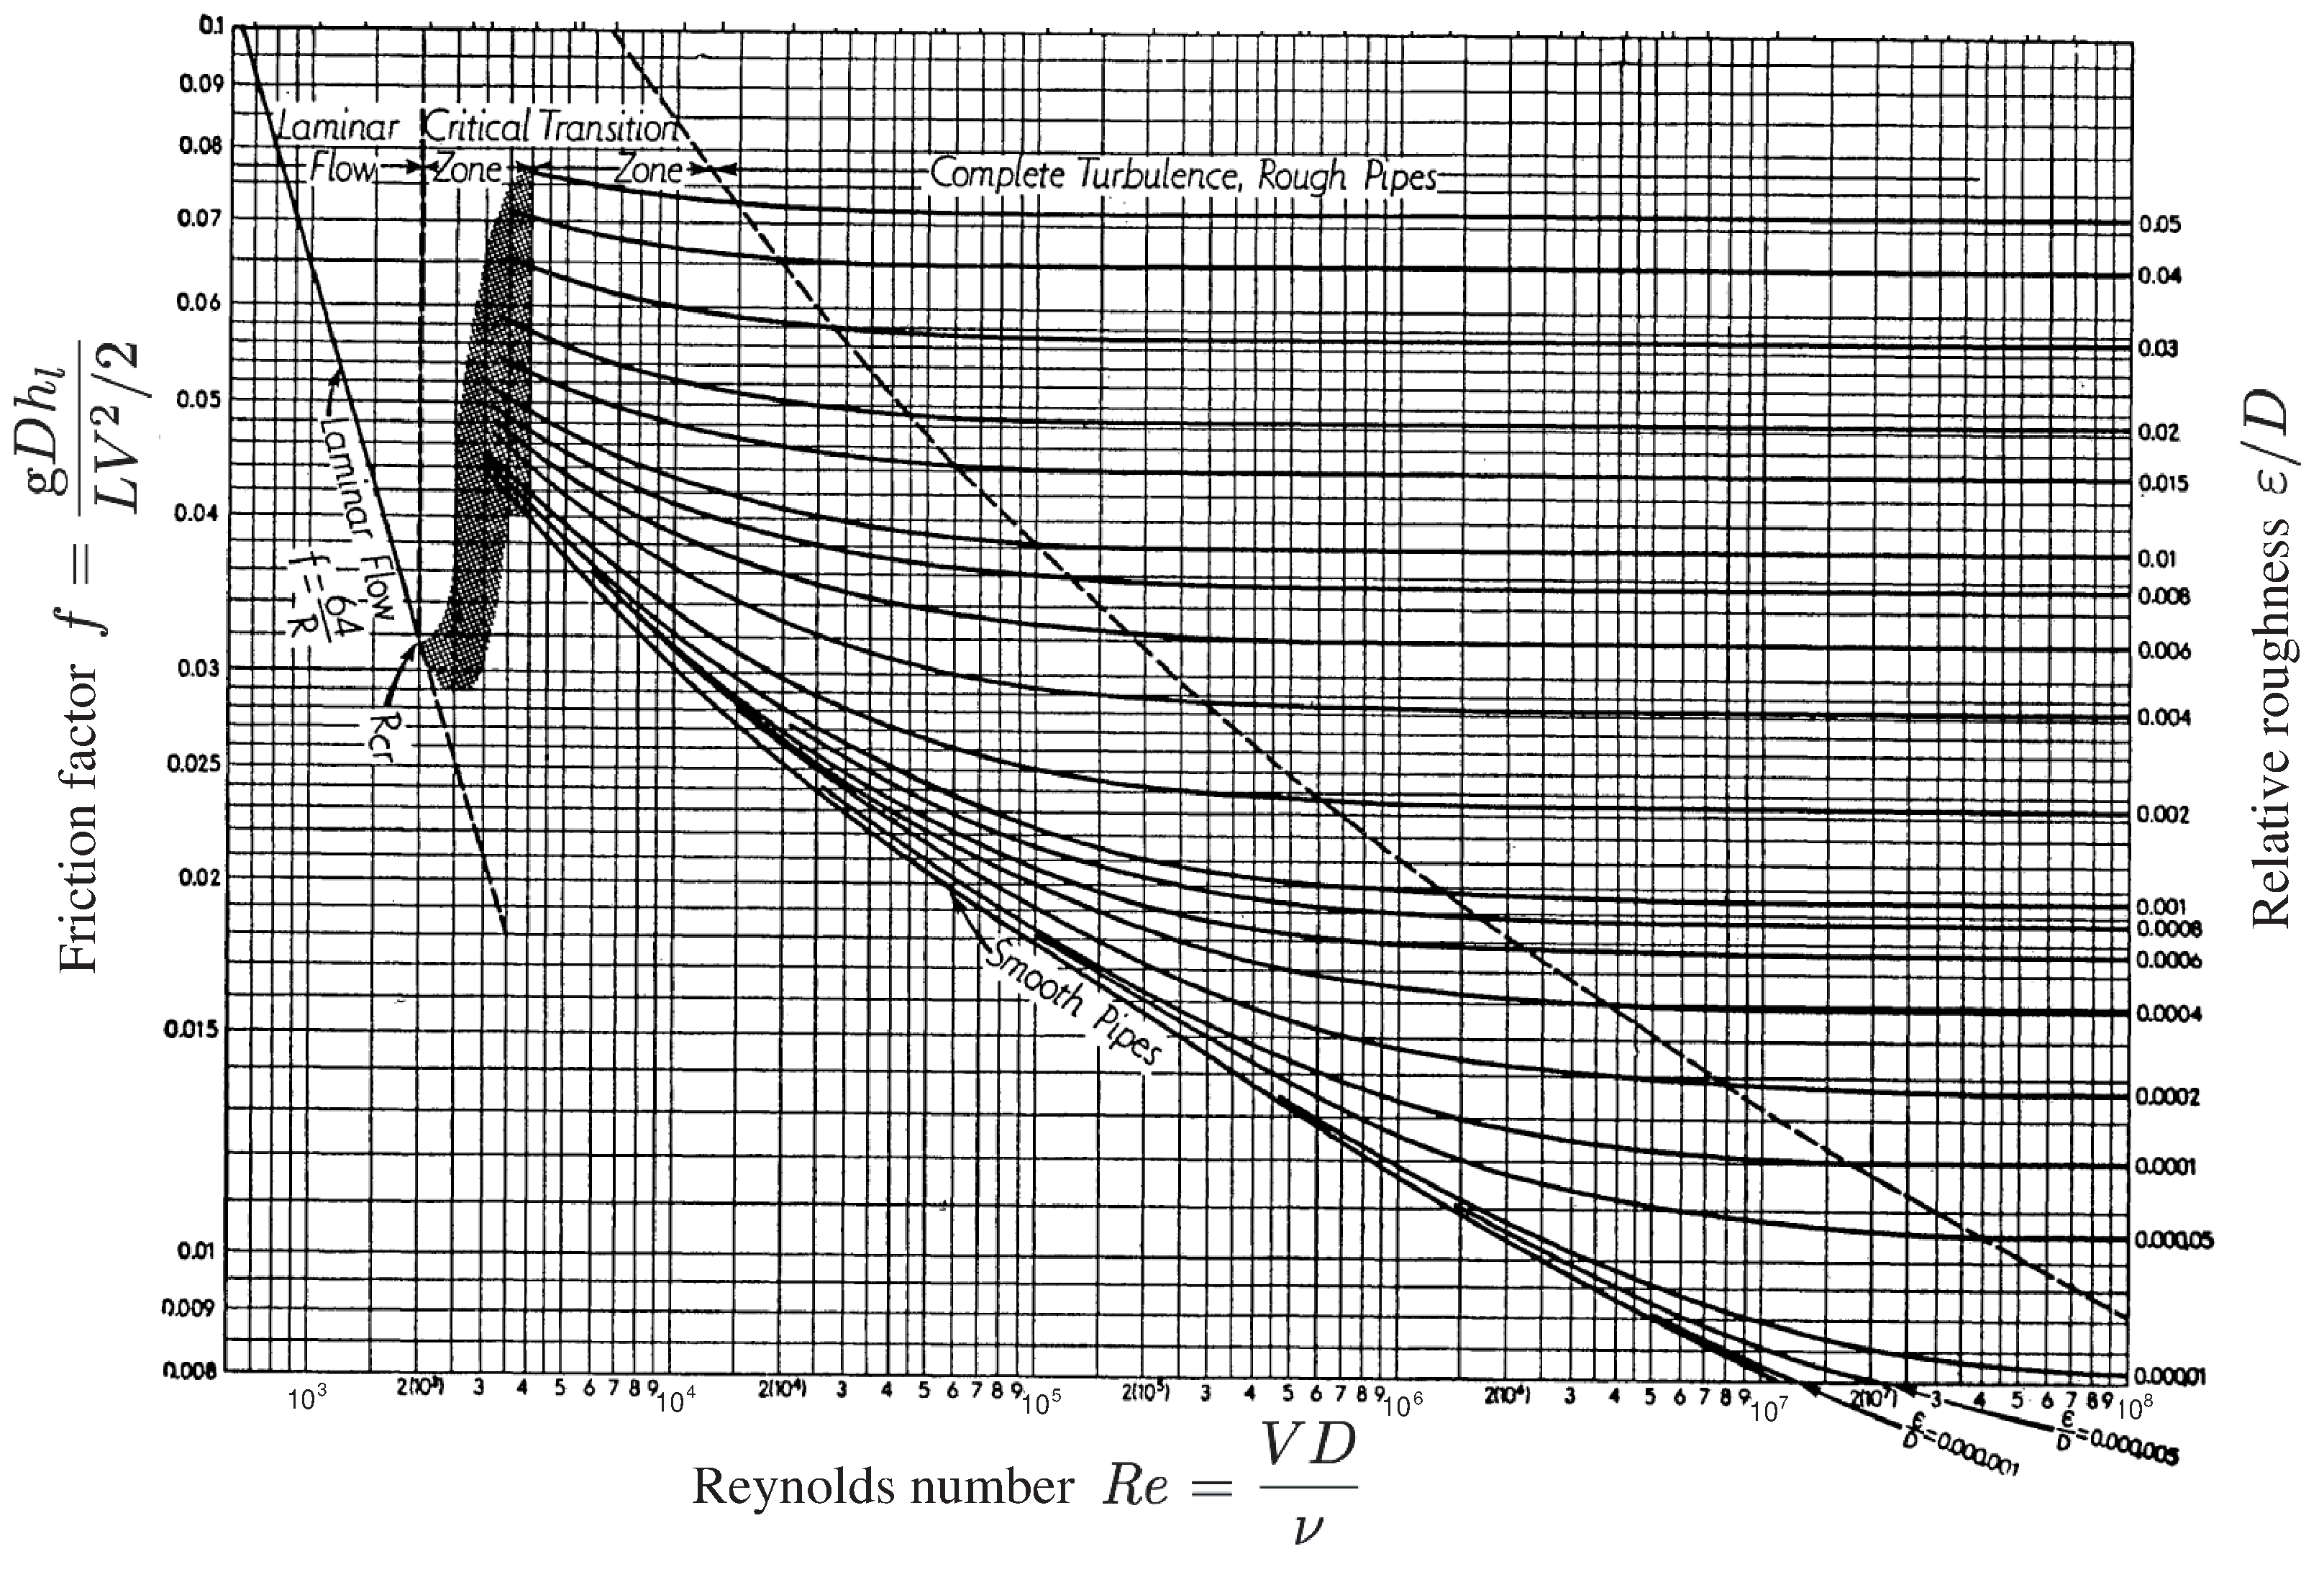
\includegraphics[angle=90,height=0.9\textheight]{MoodyChartReLabelled.eps}
\end{center}
\caption{The Moody Chart for frictional losses in pipe flow.}
\label{fig.moody}
\end{figure}


%%%%%%%%%%%%%%%%%%%%%%%%%%%%%%%%%%%%%%%%%%%%%%%%%%%%%%%%%%%%%%%%%%%%%%%%%%%%%%%
\end{document}
